\documentclass{../Vorlage/mat}
\lstset{
	basicstyle=\small
}

\begin{document}
\maketitle{Sebastian Bliefert}{}{Nils Drebing}{}{Pascal Pieper}{}{15.12.2016}{Bonus} \\

\section*{Aufgabe A}
\begin{align*}
\phi & = 2 \pi \cdot \frac{47^{\circ}}{360^{\circ}}\\
& = 0.820304748437 
\end{align*}

\subsection*{a}
\begin{align*}
z & = exp(\imath \cdot \phi)\\
& = cos(\phi) + sin(\phi)i\\
& = cos(0.820304748437) + sin(0.820304748437)i\\
z & = 0.681998360062 + 0.731353701619i
\end{align*}
\newpage

\subsection*{b}
\begin{figure}[!htb]
\centering
	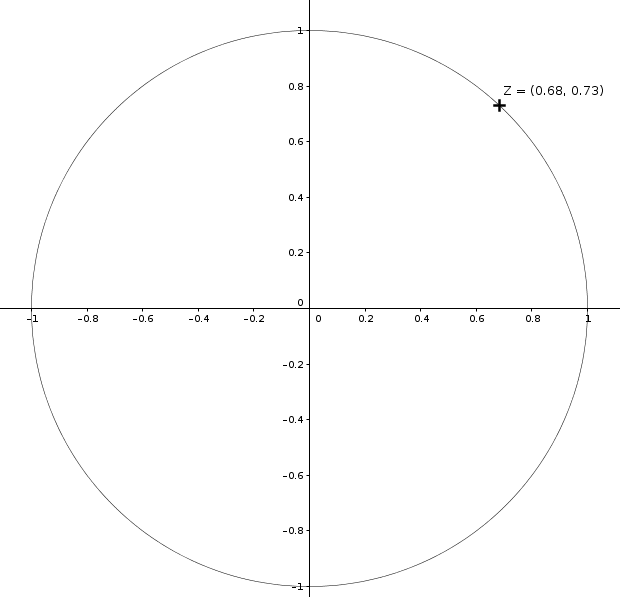
\includegraphics[scale=0.5]{circle_z.png}
	\label{circlez}
	\caption{Einheitskreis mit dem berechneten Punkt \textit{z}}
\end{figure}
\newpage

\subsection*{c}
\begin{figure}[!htb]
\centering
	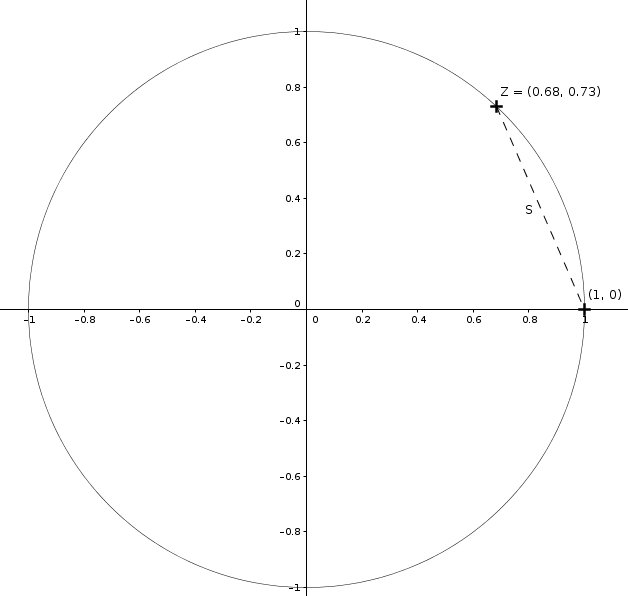
\includegraphics[scale=0.5]{circle_s.png}
	\label{circles}
	\caption{Einheitskreis mit dem berechneten Punkt \textit{z} und Strecke \textit{s} zwischen \textit{z} und $(1,0)^T$}
\end{figure}

\subsection*{d}
Nach Euklidischer Norm:
\begin{align*}
\|s\| & = \sqrt{(z_x - 1)^2 + (z_y - 0)^2}\\
& = \sqrt{(0.681998360062 - 1)^2 + 0.731353701619^2}\\
& = 0.79749813785
\end{align*}

\section*{Aufgabe B}


\section*{Aufgabe C}


\section*{Aufgabe D}
\subsection*{1}
\subsubsection*{(a)}
\begin{equation}
	R^{(1)} = \begin{pmatrix}
	0.87461971 & -0.4848092 & 0 \\
	0.4848092 & 0.87461971 & 0\\
	0&0&1
	\end{pmatrix}
\end{equation}
$q_0 = 1 + 0.87461971 + 0.87461971 + 1$\\
$q_1 = 0 - 0$\\
$q_2 = 0 - 0$\\
$q_3 = -0.4848092 - 0.4848092$\\
Also ist $\hat{q} = (3.74923942, 0, 0, -0.9696184)$
\subsubsection*{(b)}
$q_0 = \cos{\frac{\phi}{2}}$
\subsection*{2}
\begin{align*}
\phi & = 2 \pi \cdot \frac{70^{\circ}}{360^{\circ}}\\
& = 0.820304748437 
\hat{n} & = (0,1,0)^T
\end{align*}
\subsection*{(a)}
\begin{align*}
R^{(2)} & = exp(\phi \cdot \hat{n}^\otimes) = I + sin(\phi) \cdot \hat{n}^\otimes + (1 - cos(\phi)) \cdot (\hat{n}^\otimes)^2\\
& = 
\begin{pmatrix}
1 & 0 & 0 \\
0 & 1 & 0\\
0 & 0 & 1 \\
\end{pmatrix} + sin(\phi) \cdot
\begin{pmatrix}
0 & 0 & 1 \\
0 & 0 & 0 \\
-1 & 0 & 0 \\
\end{pmatrix} + (1 - cos(\phi)) \cdot
\begin{pmatrix}
0 & 0 & 1 \\   
0 & 0 & 0 \\
-1 & 0 & 0 \\
\end{pmatrix}^2 						\\
& = 
\begin{pmatrix}
1 & 0 & 0 \\
0 & 1 & 0\\
0 & 0 & 1 \\
\end{pmatrix} +
\begin{pmatrix}
0 & 0 & 0.939 \\
0 & 0 & 0 \\
-0.939 & 0 & 0 \\
\end{pmatrix} + 
\begin{pmatrix}
0 & 0 & 0.658 \\   
0 & 0 & 0 \\
0.658 & 0 & 0 \\
\end{pmatrix} 						\\
R^{(2)} & =  
\begin{pmatrix}
1 & 0 & 1.5976 \\
0 & 1 & 0\\
-0.2817 & 0 & 1 \\
\end{pmatrix}
\end{align*}
%0.939 sin 
% 1 - cos phi = 0.657979856674
\subsection*{(b)}
\begin{align*}
\hat{q} & = cos(\frac{\phi}{2}) + sin(\frac{\phi}{2}) \cdot j * \hat{n}\\
& = 0.819152 + (0.573576j,0.573576k,0.573576l)^T * (0,1,0)^T\\
\hat{q} & = (0.819152, 0, 0.573576k, 0)
\end{align*}

\end{document}
